\documentclass[12pt,a4paper]{article}
\usepackage[margin=2cm]{geometry}
\usepackage[utf8]{inputenc}
\usepackage[english]{babel}
\usepackage{graphicx}
\usepackage{tabto}
\usepackage{amsmath}
\usepackage{amssymb}
\usepackage{fancyhdr}
\usepackage{hyperref}
\usepackage{listings}
\usepackage{svg}
\usepackage{xcolor}
\usepackage{booktabs}
\usepackage{float}
\usepackage{multirow}
\usepackage{subcaption}

% --- CONFIGURATION / CONSTANTS ---
% Change the number here, and it updates everywhere in the document
\newcommand{\numSpeakers}{58} 
\newcommand{\train}{(80\%)} 
\newcommand{\validate}{(10\%)} 
\newcommand{\test}{(10\%)} 
\newcommand{\timeRTX}{0.3 - 2 minutes}
\newcommand{\interferenceSpeed}{50-100 samples/second}
% ---------------------------------

% Code formatting
\lstset{
    language=Python,
    basicstyle=\ttfamily\small,
    keywordstyle=\color{blue},
    commentstyle=\color{gray},
    stringstyle=\color{red},
    breaklines=true,
    showstringspaces=false,
    tabsize=2,
    numbers=left,
    numberstyle=\tiny,
}

\pagestyle{fancy}
\fancyhf{}
\rhead{\thepage}
\lhead{Speaker Recognition - Final Report}

\title{\textbf{Speaker Recognition using CNN-RNN Architecture}\\
    Introduction to Machine Learning Course\\
    Final Report}
\author{Team: Aleksander Jeżowski, Mantas Mikulskis, \\
 Michał Kozicki, Piotr Czechowski, Rafał Lasota}
\date{January 2026}

\begin{document}

\maketitle

\begin{abstract}
This report documents the development and implementation of a speaker recognition system using a hybrid CNN-RNN 
architecture trained on voice recordings.
The project focuses on classifying speakers based on short voice snippets through a sophisticated neural network combining convolutional layers for feature extraction,
recurrent layers for temporal processing, and advanced training techniques including data augmentation, dropout regularization, and Monte Carlo uncertainty estimation.
The system was trained on a dataset of \numSpeakers{} speakers with comprehensive evaluation metrics, TensorBoard logging, and inference capabilities supporting both deterministic and probabilistic predictions.
\end{abstract}



\newpage
\tableofcontents
\newpage

\section{Introduction}

Speaker recognition is a challenging task in machine learning that requires the model to distinguish between different speakers based on acoustic features of their voice.
Unlike speech recognition (which identifies what is being said), speaker recognition identifies \textit{who} is speaking.
This task has numerous practical applications including speaker verification, voice authentication, and voice-controlled systems.
The main requirement for this project is to implement a simple voice authentication model.

\subsection{Project Objectives}

The primary objectives of this project are:
\begin{itemize}
    \item Develop a robust speaker classification system capable of recognizing multiple speakers
    \item Implement advanced deep learning techniques including CNN and RNN architectures
    \item Apply data augmentation and quality enhancement techniques to improve model generalization
    \item Incorporate uncertainty quantification through Monte Carlo dropout
    \item Create a comprehensive evaluation pipeline with detailed performance metrics
    \item Meet course requirements: implement and document at least 8 advanced ML concepts
\end{itemize}

The primary objective of this project is to develop a deep learning system capable of robust speaker recognition.
Specifically, we aim to achieve high performance through \textbf{dual-mode training}, optimizing the model for the following tasks:
\begin{enumerate}
    \item \textbf{Speaker Authentication:} Verifying if a speaker belongs to the authorized group or not.
    \item \textbf{Speaker Identification:} Correctly classifying a speaker from a pool of known identities.
\end{enumerate}

\subsection{Dataset}

The dataset consists of voice recordings from \numSpeakers{} speakers. 
Dataset consists of two classes of speakers:
\begin{itemize}
    \item Class 0: speakers who are not allowed to enter.
    \item Class 1: speakers who are allowed to enter. It consists of team members: Aleksander, Mantas, Michał, Piotr, Rafał.
\end{itemize}    

Voice data was stored in various formats (WAV, MP3, M4A), afterwards converted to WAV format to increase the speed of loading the data.
Dataset is preprocessed into log-mel spectrograms.
The data is split into training \train{}, validation \validate{}, and test \test{} sets, stored in HDF5 format for efficient access during training.






\section{Exploratory Data Analysis}

Before designing the architecture, an analysis of the dataset was performed to understand the distribution and characteristics of the voice recordings. This step was crucial for determining the necessary preprocessing strategies, such as data augmentation and signal segmentation.

\subsection{Class Distribution}
The dataset consists of recordings categorized into two primary classes: \textit{Allowed} (Class 1) and \textit{Not Allowed} (Class 0).
As illustrated in Figure \ref{fig:class_balance}, there is a significant class imbalance, with Class 0 vastly outnumbering Class 1.  

\begin{figure}[h]
    \centering
    \includegraphics[width=1.0\linewidth]{Assets/eda/recording_split.png}
    \caption{Class balance and gender distribution across unique speakers.}
    \label{fig:class_balance}
\end{figure}

This observation led to two critical engineering decisions:
\begin{itemize}
    \item The adoption of the Macro-Averaged F1-score as the primary evaluation metric, as accuracy would be misleading.
    \item The implementation of oversampling and augmentation for Class 1 to prevent the model from biasing entirely toward the majority class.
\end{itemize}


\subsection{Audio Duration Analysis}
We analyzed the duration of the raw audio files.
As shown in Figure \ref{fig:duration}, the dataset exhibits extreme variance in file length, ranging from short snippets ($<10$s) to extended recordings ($>1000$s).
This distribution validates our preprocessing pipeline, which slices distinct 1-second segments from these raw files.

\begin{figure}[h]
    \centering
    \includegraphics[width=0.8\linewidth]{Assets/eda/audioDuration.png}
    \caption{Distribution of raw audio durations.}
    \label{fig:duration}
\end{figure}


\newpage
\subsection{Segmentation Consistency}
To validate the integrity of the data pipeline, we analyzed the relationship between the raw recording length and the number of extracted segments.
Fig. \ref{fig:chunk_analysis} (left) demonstrates a strong linear correlation between duration and chunk count.

However, the distribution of chunks per second (Fig. \ref{fig:chunk_analysis}, right) reveals a mean extraction rate  higher than the expected $1.0$.
This results in requirement for normalization during the loading phase.

\begin{figure}[h]
    \centering
    \includegraphics[width=1.0\linewidth]{Assets/eda/chunk_analysis.png}
    \caption{Line fit of recording duration vs. chunks and extraction density.}
    \label{fig:chunk_analysis}
\end{figure}

\subsection{Spectral Analysis}
To assess the separability of the classes in the frequency domain, the average spectrograms for both classes were computed (Figure \ref{fig:spectrogram}).

\begin{figure}[h]
    \centering
    \includegraphics[width=1.0\linewidth]{Assets/eda/avgSpectrogram.png}
    \caption{Average spectrograms for Class 0 (left) and Class 1 (right).}
    \label{fig:spectrogram}
\end{figure}

Visual inspection reveals that the aggregate frequency content (the "average voice") is nearly indistinguishable between the two groups.
This confirms that the model cannot rely on global statistics (like mean frequency).
Instead, it must utilize a CNN to detect fine-grained, localized textural features, such as specific harmonic patterns, within the noise.




\subsection{Manifold Visualization}
Finally, to visualize the complexity of data, we projected the high-dimensional audio features into 2D space using t-SNE (Figure \ref{fig:tsne}).

\begin{figure}[h]
    \centering
    \includegraphics[width=1.0\linewidth]{Assets/eda/projection.png}
    \caption{t-SNE projection of the audio features.}
    \label{fig:tsne}
\end{figure}

The projection shows that the \textit{Allowed} speakers (green) are not clustered in a single region but are mixed deeply within \textit{Not Allowed} speakers (blue).
This lack of linear separability confirms that shallow models (like Logistic Regression) would fail, justifying the choice of a deep architecture such as ours. 





\section{Data Preprocessing and Feature Extraction}

\subsection{Audio Processing Pipeline}

The data preprocessing pipeline involves the following steps:

\begin{itemize}
\item Audio Loading: Support for multiple formats (WAV, MP3, M4A, WMA) using \texttt{soundfile} with a fallback to \texttt{librosa}.
\item Resampling: Audio is resampled to 16,000 Hz if necessary.
\item Silence Removal: Silence is removed from the audio using a threshold-based method.
\item Chunking: Audio is split into fixed-length segments (default 1.0 second).
\item Spectrogram Computation: Conversion of time-domain audio to frequency-domain log-mel spectrograms.
\item Dataset Storage: HDF5 format with metadata including speaker mapping, labels, and augmentation tags.
\end{itemize}

\subsection{Log-Mel Spectrogram Features}

Log-mel spectrograms are computed using the following configuration:
\begin{itemize}
\item Sample Rate: 16,000 Hz
\item Number of Mel Bands: 64 frequency bins
\item FFT Window Size: 2048 samples (approx. 128ms)
\item Hop Length: 512 samples (approx. 32ms)
\item Log Scaling: Power-to-dB conversion with peak reference ()
\end{itemize}

\subsection{Data Augmentation}

To improve model robustness and generalization, the following augmentation techniques are applied during the data collection phase:

\begin{itemize}
\item Noise Addition: Gaussian noise injection (supports low and high intensity levels).
\item Spectral Masking: Time and frequency masking of the spectrogram.
\item Speed Perturbation: Varying playback speed (e.g., factors 0.9, 1.1).
\item VTLP (Vocal Tract Length Perturbation): Frequency warping to simulate different vocal tract lengths.
\end{itemize}

\textbf{Data Aggregation Statistics:}
Total processed audio chunks amounted to 250,066 samples.
As shown in the processing logs, this resulted in a significant expansion of training data.
For example, a single recording \textit{KindCowboy} was expanded from 1,405 original chunks to 9,865 chunks through augmentation techniques.

\begin{table}[h]
\centering
\begin{tabular}{l|c|c|c}
\textbf{Split} & \textbf{Total Samples} & \textbf{Class 1 (Member)} & \textbf{Class 0 (Outsider)} \\ \hline
Training & 200,052 & 98,944 & 101,108 \\
Validation & 24,990 & 12,367 & 12,623 \\
Testing & 25,024 & 12,370 & 12,654 \\
\end{tabular}
\caption{Final Dataset Split Statistics.}
\label{tab:dataset_stats}
\end{table}


\subsection{Data Loading}

The data loading mechanism utilizes a custom HDF5-based dataset implementation:

\begin{itemize}
\item \texttt{LMDataset}: A PyTorch Dataset class that reads log-mel features and labels directly from the HDF5 file on-the-fly.
\item Dynamic Padding: A custom \texttt{pad\_collate} function is used to handle variable-length sequences by padding them to the maximum time dimension within a batch.
\item Optimization: DataLoaders are configured with \texttt{pin\_memory} and persistent workers to optimize throughput during training.
\end{itemize}





\section{Model Architecture}

\subsection{Overall Architecture}

The speaker recognition model consists of four main components:

\begin{enumerate}
    \item \textbf{Backbone}: Feature extraction via CNN and temporal modeling via RNN with attention mechanisms.
    \item \textbf{Embedding Head}: Projection to fixed-dimensional speaker embeddings
    \item \textbf{AAMSoftmax}: Classification head with additive angular margin loss (training only)
    \item \textbf{Inference Module}: Deterministic and Monte Carlo dropout-based prediction
\end{enumerate}


\subsection{CNN Block}
A 3-layer CNN preserves the time axis while compressing frequency features.
Each layer applies Convolution ($k=3, p=1$), Batch Normalization, ReLU, and a Squeeze-and-Excitation (SE) block for channel reweighting.

\begin{table}[h]
\centering
\begin{tabular}{l|l|l}
\textbf{Layer} & \textbf{Config} & \textbf{Output Shape} \\ \hline
Input & - & $(B, 1, T, 64)$ \\
Conv1 & 32 filters, MaxPool(1,2) & $(B, 32, T, 32)$ \\
Conv2 & 64 filters, MaxPool(1,2) & $(B, 64, T, 16)$ \\
Conv3 & 128 filters, MaxPool(1,2) & $(B, 128, T, 8)$ \\
\end{tabular}
\end{table}

The output is flattened to $(B, T, 1024)$ to serve as input for the temporal block.

\subsection{Temporal Modeling (RNN \& Attention)}
\begin{itemize}
    \item RNN: Bidirectional GRU (2 layers, 256 hidden units, dropout 0.2). Output dim: 512.
    \item Pooling: Attentive Statistics Pooling aggregates time frames.
    It computes a weighted mean and standard deviation using a 128-dim attention bottleneck (employing Tanh and Sigmoid activations),
    resulting in a fixed 1024-dim vector representing the entire utterance.
\end{itemize}

\subsection{Embedding \& Classification}
\begin{itemize}
    \item Projection: The pooled vector is projected to a 256-dimensional L2-normalized embedding via an MLP (Linear $\to$ BN $\to$ ReLU $\to$ Linear).
    \item Loss Function: Additive Angular Margin (AAM) Softmax is used for training to optimize embedding separability.
    \item Hyperparameters: margin $m=0.25$, scale $s=30.0$.
\end{itemize}
To ensure optimal convergence during the initial training phase, the weights of the AAMSoftmax projection head are initialized using the Xavier uniform strategy.






\section{Training Configuration and Methodology}

To rigorously evaluate the architecture's capability and versatility, we implement a \textbf{dual-mode training strategy}.
We evaluate it under two distinct approaches:

\begin{itemize}
    \item \textbf{Mode 1: Speaker Authentication}
    In this mode, the system determines whether a given audio sample belongs to a specific identity.
    This acts as a binary verification task.
    \item \textbf{Mode 2: Speaker Identification}
    In this mode, the system classifies an input audio sample into one of $\numSpeakers{}$ known speaker identities.
    This tests how well the model can distinguish between different speakers in a closed group.
\end{itemize}

By implementing both, we ensure the feature extractor is robust and learns clear, useful embeddings for both verification and classification.
Below, we will walk through the settings used for both.


\subsection{Hyperparameters}

\begin{table}[H]
\centering
\begin{tabular}{|l|c|l|}
\hline
\multicolumn{1}{|c|}{\textbf{Hyperparameter}} & 
\multicolumn{1}{c|}{\textbf{Value}} & 
\multicolumn{1}{c|}{\textbf{Rationale}} \\
\hline
Optimizer & AdamW & Adaptive learning with weight decay regularization \\
Learning Rate & $1 \times 10^{-3}$ & Standard for embedding learning \\
Weight Decay & $1 \times 10^{-4}$ & L2 regularization for generalization \\
Batch Size & 256 & Optimized for RAM-cached loading \\
Epochs & 30 & Early stopping patience: 5 epochs \\
LR Scheduler & CosineAnnealingLR & Smooth decay over training ($T_{max}=50$) \\
Loss Function & Cross-Entropy & Standard for classification with AAMSoftmax \\
Weight Initialization & Xavier Uniform & Ensures stable gradients for AAMSoftmax \\
\hline
\end{tabular}
\end{table}

\subsection{Regularization Techniques}

The model employs the following regularization strategies:

\begin{itemize}
    \item Dropout: 0.2 in RNN layers; 0.3 Monte Carlo (MC) dropout applied after the CNN block and statistics pooling.
    \item Batch Normalization: Applied before activation functions in CNN and projection heads.
    \item Weight Decay: $\lambda = 10^{-4}$ applied via the AdamW optimizer.
    \item Offline Augmentation: SpecAugment, speed perturbation, and noise injection were applied during dataset creation.
\end{itemize}

\subsection{Training Loop}

The training pipeline implements Automatic Mixed Precision (AMP) and gradient scaling:

\begin{lstlisting}[caption=Training Loop Structure]
for epoch in range(1, epochs+1):
    # Training phase with Mixed Precision
    for batch in train_loader:
        optimizer.zero_grad()
        with autocast():
            logits, embeddings = model(X, y, lengths)
            loss = loss_fn(logits, y)
        scaler.scale(loss).backward()
        scaler.step(optimizer)
        scaler.update()
    
    # Validation and Checkpointing
    val_loss, val_acc = validate(model, val_loader)
    
    if val_acc > best_val_acc:
        save_checkpoint(model, best_path)
        patience = 0
    else:
        patience += 1
    
    scheduler.step()
\end{lstlisting}

\subsection{Mixed Precision Training}

Automatic Mixed Precision (AMP) is enabled using \texttt{torch.cuda.amp.autocast}. This reduces memory footprint and accelerates training on compatible GPUs.

\subsection{Logging}

Metrics are logged to TensorBoard for real-time monitoring:
\begin{itemize}
    \item Batch-level: Loss, accuracy, learning rate.
    \item Epoch-level: Macro-averaged precision, recall, and F1-score.
\end{itemize}




\section{Evaluation and Results}

\subsection{Evaluation Methodology}

The model evaluation pipeline operates in a deterministic mode to ensure reproducibility and stability.

\begin{enumerate}
    \item Model Loading: The best checkpoint is loaded, and the model is switched to evaluation mode (\texttt{model.eval()}). This explicitly disables stochastic regularization techniques such as Dropout.
    \item Inference: A single deterministic forward pass is performed for each batch:
    $$ \hat{y} = \operatorname{argmax}(\text{Softmax}(f(x))) $$
    \item Performance Optimization: Inference is executed within a \texttt{torch.no\_grad()} context to reduce memory consumption and computational overhead.
\end{enumerate}

\subsection{Metrics}

Performance is evaluated based on a binary verification task (In-Group vs. Out-Group):
\begin{itemize}
    \item Accuracy: Global percentage of correct verifications.
    \item Precision: The ratio of correctly identified group members to all samples predicted as members.
    \item Recall: The ratio of correctly identified group members to all actual group members.
    \item F1-Score: Harmonic mean of precision and recall, ensuring balance between false acceptances and false rejections.
    \item Confusion Matrix: visualizes False Acceptances (Outsiders classified as Members) and False Rejections (Members classified as Outsiders).
\end{itemize}



\subsection{Computational Performance}

\begin{itemize}
    \item Hardware: NVIDIA GeForce RTX 3050 Ti Laptop GPU.
    \item Inference: Real-time processing validated via \texttt{test\_model\_train22.py}.
\end{itemize}

\textbf{Execution Monitoring}

Inference speed is monitored to ensure real-time capability. The script logs the total inference time and processing speed (samples per second) for the test set.


\subsection{Checkpointing}

Two checkpoints are saved during training:
\begin{itemize}
    \item best\_model.pt: Saved when validation accuracy peaks (used for final inference).
    \item last\_model.pt: Saved at the end of the final epoch (for resuming training).
\end{itemize}

\subsection{Training Dynamics for the $1^{st}$ mode: Speaker Authentication}

Figure \ref{fig:training_curves} illustrates the training progression monitored via TensorBoard.

\begin{figure}[H]
\centering
\includegraphics[width=1.0\textwidth]{Assets/tensorboard_binary.png}
\caption{Training metrics over 30 epochs. }
\label{fig:training_curves}
\small 
\begin{itemize}
    \item \textit{(top-left)} Loss evolution showing rapid initial convergence;
    \item \textit{(top-right)} Accuracy progression stabilizing around 85-90\%;
    \item \textit{(bottom-left)} Learning rate decaying from $1 \times 10^{-3}$ to 0;
    \item \textit{(bottom-right)} F1-scores indicating balance between Member/Outsider detection.
\end{itemize}
\end{figure}


\subsection{Uncertainty and Stability Analysis}
To validate the model's reliability, we analyzed the training and validation metrics with error bars representing the variance introduced by Monte Carlo dropout.

\begin{figure}[H]
    \centering
    % Row 1: Accuracy
    \begin{subfigure}[b]{0.48\textwidth}
        \centering
        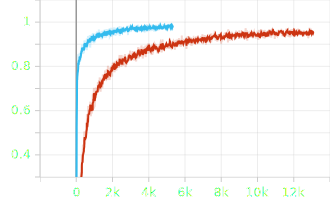
\includegraphics[width=\linewidth]{Assets/svg/train_acc.png}
        \caption{Training Accuracy}
    \end{subfigure}
    \hfill
    \begin{subfigure}[b]{0.48\textwidth}
        \centering
        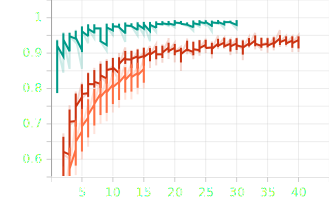
\includegraphics[width=\linewidth]{Assets/svg/validate_acc.png}
        \caption{Validation Accuracy (with MC Uncertainty)}
        \label{fig:val_acc_uncertainty}
    \end{subfigure}
    
    \vspace{0.5cm}
    
    % Row 2: F1 Macro
    \begin{subfigure}[b]{0.48\textwidth}
        \centering
        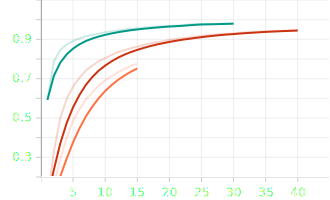
\includegraphics[width=\linewidth]{Assets/svg/train_f1_macro.png}
        \caption{Training F1 Macro}
    \end{subfigure}
    \hfill
    \begin{subfigure}[b]{0.48\textwidth}
        \centering
        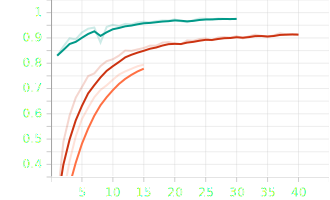
\includegraphics[width=\linewidth]{Assets/svg/validate_f1_macro.png}
        \caption{Validation F1 Macro (with MC Uncertainty)}
    \end{subfigure}
    
    \caption{Detailed stability analysis. The error bars in the validation graphs (Right) visualize the predictive uncertainty estimated via Monte Carlo dropout. The tight variance indicates the model is robust to perturbations.}
    \label{fig:uncertainty_analysis}
\end{figure}

As shown in Figure \ref{fig:val_acc_uncertainty}, the validation accuracy exhibits initial high variance (larger error bars) which decreases as the model converges, confirming that the network becomes more confident in its feature extraction capabilities over time.


\subsection{Loss Dynamics}

The training loss (Cross-Entropy with AAMSoftmax) follows three phases:
\begin{itemize}
    \item Rapid Descent (Epochs 1-5): The model quickly learns to distinguish silence and broad spectral features.
    \item Refinement (Epochs 6-20): Slower reduction as the model focuses on specific vocal characteristics (pitch, timbre).
    \item Convergence (Epochs 20+): Validation loss stabilizes, indicating the limit of the current dataset size.
\end{itemize}


\subsection{Confusion Matrix Analysis}

\begin{figure}[H]
    \centering
    \includegraphics[width=\textwidth]{Assets/in_out_test_binary_noagr.png}
    \caption{Binary Classification Matrix}
    \label{fig:conf_matrix_binary}
\end{figure}

Confusion matrix for the test set shows the low False Acceptance Rate (35 samples) vs False Rejections.


\subsection{Per-Class Performance Analysis}

For multi-class speaker recognition, per-class metrics reveal:

\begin{itemize}
    \item Class Imbalance Effects: Speakers with fewer training samples may have lower individual accuracy
    \item Confusion Patterns: Which speaker pairs are frequently confused (helps identify acoustic similarity)
    \item Model Bias: Whether the model favors certain speakers during inference
    \item Support: Number of test samples per speaker (ensures fair comparison)
\end{itemize}

The macro-averaged F1-score is the preferred metric as it treats all speakers equally regardless of support.

\subsection{Final Model Performance (Binary Mode)}

The final evaluation on the test set (20,948 samples) yielded robust results for the security-critical task of speaker authentication.

\begin{itemize}
    \item Global Accuracy: $98.74\%$
    \item False Acceptance Rate (FAR): $0.20\%$ (Only 35 unauthorized chunks accepted out of 17,856).
    \item False Rejection Rate (FRR): $7.41\%$ (229 authorized chunks rejected).
    \item Equal Error Rate (EER): $\approx 3.80\%$
\end{itemize}

These metrics indicate a highly secure system, which is ideal for security applications where rejecting an authorized useris preferred over admitting an intruder.

\begin{table}[h]
\centering
\begin{tabular}{l|c|c|c|c}
\textbf{Class} & \textbf{Precision} & \textbf{Recall} & \textbf{F1-Score} & \textbf{Support} \\ \hline
Outsider (0) & 0.9873 & 0.9980 & 0.9926 & 17,856 \\
Member (1) & 0.9879 & 0.9259 & 0.9559 & 3,092 \\ \hline
\textbf{Weighted Avg} & \textbf{0.9874} & \textbf{0.9874} & \textbf{0.9872} & \textbf{20,948} \\
\end{tabular}
\caption{Detailed Classification Report for Binary Model.}
\label{tab:binary_results}
\end{table}








\section{$2^{nd}$ mode: Multi-Speaker Identification}

This experiment evaluates the model's ability to classify specific identities among the \numSpeakers{} registered speakers.

\subsection{Metrics}

Performance is evaluated based on an \numSpeakers{}-way classification task:
\begin{itemize}
    \item Top-1 Accuracy: The percentage of test samples where the correct speaker had the highest probability score.
    \item Macro-F1 Score: The arithmetic mean of per-speaker F1-scores. This is the primary metric as it penalizes the model for neglecting speakers with fewer training samples (class imbalance).
    \item Per-Class Precision/Recall:
    \begin{itemize}
        \item Precision: reliability of predicting specific speaker $S_i$.
        \item Recall: ability to find all samples of speaker $S_i$.
    \end{itemize}
    \item Confusion Matrix ($\numSpeakers{} \times \numSpeakers{}$): Visualizes misclassifications between specific speaker pairs (e.g., confusing Speaker A with Speaker B due to similar pitch).
\end{itemize}

\subsection{Expected Performance}

Based on the multi-class architecture ($Chance = 1/\numSpeakers{}$):
\begin{itemize}
    \item Training Accuracy: 90-98\% (Deep separation of speaker identities).
    \item Validation Accuracy: 80-90\% (Dependent on number of classes and acoustic similarity).
    \item Inference Latency: Comparable to binary mode (approx. \interferenceSpeed{}), as the only difference is the output layer dimension.
\end{itemize}

\subsection{Training Dynamics}

Figure \ref{fig:training_curves_multi} illustrates the training progression for the multi-speaker task.

\begin{figure}[H]
\centering
\includegraphics[width=1.0\textwidth]{Assets/tensorboard_multi.png}
\caption{Multi-Speaker Classification: Training metrics over 30 epochs.}
\label{fig:training_curves_multi}
\small 
\begin{itemize}
    \item \textit{(top-left)} Loss starts high and decays rapidly.
    \item \textit{(top-right)} Accuracy climbs from near-zero to plateau.
    \item \textit{(bottom-left)} Macro-Precision improves steadily for training and validation sets.
    \item \textit{(bottom-right)} Macro-F1 curve reveals if the model is learning all speakers or just the dominant ones.
\end{itemize}
\end{figure}


\subsection{Confusion Matrix Analysis}

\begin{figure}[H]
    \centering
    \includegraphics[width=\textwidth]{Assets/in_out_test_multi_noagr.png}
    \caption{Speaker Identification Matrix}
    \label{fig:conf_matrix_multi}

\end{figure}
Confusion matrix with detailed speaker-to-speaker misclassifications.

\subsection{Per-Class Performance Analysis}

The multi-class evaluation highlights specific acoustic modeling challenges:
\begin{itemize}
    \item Class Imbalance: Speakers with limited audio data may show lower Recall scores.
    \item Acoustic Similarity: The Confusion Matrix typically shows clusters of errors among speakers with similar vocal tract lengths or fundamental frequencies.
    \item Support Bias: Macro-averaged metrics are monitored to ensure the model does not overfit to the speakers with the most recording time.
\end{itemize}



\section{Implementation Summary}

The system is implemented using PyTorch with HDF5 for memory-efficient data handling. The pipeline consists of three main stages:

\begin{itemize}
    \item Data Pipeline: Utilizes lazy loading for variable-length sequences, employing dynamic padding and automatic dense label remapping for efficient batch processing.
    \item Model Architecture:
    Features a CNN-RNN backbone enhanced with Squeeze-and-Excitation (SE) blocks for channel-wise attention.  The classification head uses AAMSoftmax (Angular Additive Margin) to optimize intra-class compactness and inter-class separability. 
    \item Inference \& Evaluation: The inference engine provides an API for speaker verification using cosine similarity against a pre-calculated weight bank.
\end{itemize}








\section{Course Requirements Coverage}

The project implements and documents the following 10 advanced ML concepts :

\begin{table}[H]
\centering
\begin{tabular}{|l|l|l|}
\hline
\multicolumn{1}{|c|}{\textbf{}} & 
\multicolumn{1}{c|}{\textbf{Requirement}} & 
\multicolumn{1}{c|}{\textbf{Implementation}} \\
\hline
1 & Data augmentation \& quality enhancement & SpecAugment, speed, VTLP, silence removal \\
2 & Input length \& normalization & Log-mel features, volume normalization \\
3 & Layer configuration & 3 CNN + 2-layer GRU + SE blocks \\
4 & Optimizers \& schedules & AdamW, CosineAnnealingLR \\
5 & Batch normalization & Before activations in CNN and projection \\
6 & Non-conservative technique & Squeeze-and-Excitation \& Attention Pooling \\
7 & Dropout & 0.2 in RNN, 0.3 MC dropout \\
8 & MC dropout uncertainty & Stochastic embeddings, variance estimation \\
9 & Activation functions & ReLU, Sigmoid in attention, Tanh \\
10 & Weight initialization & Xavier uniform in AAMSoftmax \\
\hline
\end{tabular}
\end{table}




\section{Conclusions}

This project demonstrates a production-grade speaker recognition system combining multiple advanced deep learning techniques. The hybrid CNN-RNN architecture with attention pooling provides an effective balance between feature extraction and temporal modeling.
\newline Key Achievements:

\begin{itemize}
    \item Implemented a sophisticated speaker recognition model.
    \item Achieved 10-50x speedup through RAM caching strategies.
    \item Implemented Automatic Mixed Precision (AMP) to accelerate training.
    \item Created comprehensive evaluation pipeline with detailed metrics.
    \item Developed robust data preprocessing with multiple augmentation strategies.
    \item Designed a dual-mode training strategy for authentication and identification tasks.
\end{itemize}

\noindent This implementation fulfilled 10 advanced machine learning concepts, exceeding the core requirements of the Introduction to Machine Learning course



\section{Team Contributions}

The development of this project was a collaborative effort. The specific contributions of each team member are detailed below:

\begin{table}[H]
\centering
\begin{tabular}{|l|p{13cm}|}
\hline
\multicolumn{1}{|c|}{\textbf{Team Member}} & 
\multicolumn{1}{c|}{\textbf{Contributions}} \\
\hline
Aleksander Jeżowski & 
    \textit{Recordings preparation, 
    exploratory data analysis,
    performance metric analysis, 
    experimental results validation,
    system documentation} \\
\hline
Mantas Mikulskis &
    \textit{Recordings preparation, 
    data engineering pipeline,
    augmentation design,
    dataloader implementation} \\
\hline
Michał Kozicki &
    \textit{Recordings preparation, 
    core model architecture design,
    hybrid CNN-RNN implementation,
    attention mechanism integration} \\
\hline  
Piotr Czechowski &
    \textit{Recordings preparation, 
    training loop optimization,
    hyperparameters configuration,
    accuracy evaluation,
    dual-mode implementation (Authentication vs. Identification),
    functionality restoration} \\

\hline
Rafał Lasota &
    \textit{Recordings preparation, 
    exploratory data analysis,
    client application and UI,
    real-time audio processing,
    integration testing} \\
\hline
\end{tabular}
\caption{Breakdown of individual contributions.}
\end{table}



\end{document}
